% testando se a classe é lida
%\documentclass{abnt}
%\usepackage[brazil]{babel}  % pt_BR hifenization  
%\usepackage[utf8]{inputenc}  % Allow direct edition with brazilian characters.
%\usepackage[abnt-alf]{abntcite}
%\usepackage{graphicx}

\documentclass[pnumabnt,normaltoc,espacoumemeio,capchap]{abnt}		
\usepackage[brazil]{babel}
\usepackage[utf8]{inputenc}
\usepackage{abnt-alf}
\usepackage{graphicx}
\usepackage{ufc}
\usepackage{multicol}
\usepackage{listings}
\usepackage{eufrak}
\usepackage{subfig}
\usepackage[T1]{fontenc}

% Informações institucionais
\centro{Centro de Ciências}
\departamento{Campus de Quixadá}
\curso{Sistemas de Informação}
\instituicao{Universidade Federal do Ceará}

\tipotrabalho{Monografia}
\autor{Zarathon Lopes Viana}
\autorr{VIANA, Z. L.}
\titulo{Ferramenta de Apoio ao Ensino de Fundamentos de Programação baseada em TDD}
\orientador{Prof. Msc. Camilo C. Almendra} 
\instituicao{Universidade Federal do Ceará}
\local{Quixadá, Ceará}
\cidade{Quixadá}
\data{2013}
\begin{document}
\capa
\folhaderosto

%%% DEDICATORIA %%%
\pretextualchapter{Dedicatória}
	\par Dedico este trabalho a minha família, amigos, e especialmente a minha namorada. Obrigado pela paciência e pela convivência...


%%% Agradecimentos %%%
\pretextualchapter{Agradecimentos}
	\par Aos mestres e a todos que, direta ou indiretamente, contribuíram para a realização deste trabalho.


%%% Epigrafe %%%
\pretextualchapter{Epígrafe}
	\par "Você pode encarar um erro como uma besteira a ser esquecida, ou como um resultado que aponta uma nova direção." \emph{Steve Jobs}


%%% Lista de Figuras %%%
\listadefiguras

%%% SUMARIO %%%
\sumario


%%% INTRODUCAO %%%
\chapter{Introdução}
\par Cada vez mais a tecnologia avança e com isso mercados de trabalhos não param de aparecer. É cada vez maior o número de instituições de ensino superior que abrem cursos na área de computação, pois a demanda aumenta a cada dia.
\par Os alunos ao se depararem com as primeiras disciplinas que envolvem programação nas instituições de ensino superior (IES) de computação demonstram uma certo espanto, são várias as novidades: uma nova linguagem, uma nova forma de raciocinar, o uso das sintaxes das linguagens de programação, as ferramentas de software que na sua maioria são em outro idioma, assim como outras. Como consequência disso, há altos índices de reprovação nessas disciplinas, muitos alunos, desmotivam-se do curso e até mesmo ocorre evasão por conta dessa frustração de não compreender o que o professor está passando em sala de aula \cite{SI11}.
\par De acordo com uma entrevista realizada com os professores que ministram regularmente as disciplinas do ciclo básico, os alunos apresentam um raciocínio lógico mal formado e uma base matemática deficitária, condição que afeta a aprendizagem de fundamentos de programação. Estes professores não entendiam e ainda não entendem por completo o porque de uma turma não conseguir progredir.  
\par Os problemas computacionais mostram-se muitas vezes difíceis para os alunos por causa de seu tamanho e complexidade. Muitas linhas de código precisam ser escritas antes de receber qualquer retorno positivo. Isso pode ser frustrante para os alunos iniciantes, e entediante para alunos avançados.
\par A ideia desse projeto é elaborar uma maneira diferente de abordar esse tema apresentado acima, promovendo aos alunos mais práticas de programação e aos professores um feedback, quase que imediato, sobre a situação da turma. Com isso espera-se que os alunos estariam ganhando com relação a estarem exercitando constantemente a programação e os professores estariam avaliando ao mesmo tempo o progresso, ou falhas, dos alunos, podendo propor-lhes em pronto ato, uma nova explicação ou reforço do conteúdo.
\par O principal foco dessa abordagem será a adoção de Test Driven Development (TDD) ou Desenvolvimento Guiado a Teste. Esse método basicamente consiste em elaborar primeiros os testes e depois construir um programa que faça com que os testes elaborados sejam satisfeitos. O programador ou aluno consegue com isso atingir dois objetivos: primeiro, ele consegue saber o que está sendo solicitado, segundo, ele terá uma maior compreensão do que está fazendo, desenvolvendo assim o seu raciocínio lógico para resolver problemas computacionais.
\par Este trabalho guia o aluno à aprender a sintaxe básica, capaz de confirmar de forma independente, quando completou com sucesso um exercício. Vale lembrar que o aluno irá gradualmente entender a sintaxe e compreender a solução do problema. A ideia com o uso do TDD é fazer com que o aluno caminhe em passos de bebês (baby steps), faça pouco, tenha sucesso, se motive e prossiga com o resto da implementação \cite{TF12}.
\par Nesse projeto foi adaptado o método de desenvolvimento de software TDD para o ensino. Como consequência dessa abordagem também trabalhei na elaboração de uma ferramenta para apoiar essa nova forma de ensinar, todas as disciplinas que a utilizarem, no final da disciplina, mostrará a evolução do aluno. Outro ponto bastante relevante a considerar é que a parte conceitual, não será descartada, ou menos valorizada, a ferramenta disponibiliza todo o conteúdo conceitual, dividido por tópicos para que o aluno consulte quando achar necessário.


%%% Revisao Bibliografica %%%
\chapter{Revisão Bibliográfica}
\par A disciplina de fundamentos de programação é um componente curricular para o aluno que ingressa em cursos da área de tecnologia. Em nível de introdução dos fundamentos de programação, faz parte do conteúdo pragmático primeiramente em passar aos alunos uma base necessária para o desenvolvimento da lógica de programação e da representação do raciocínio através de algoritmos nexos e corretos. Essa disciplina é necessária em muitas outras disciplinas que virão pela frente durante sua vida acadêmica na área de tecnologia.
\section{A problemática do ensino de fundamentos de programação}
\par O ensino de programação de computadores aos alunos tem como principal objetivo que o mesmo aprenda a construir programas e sistemas computadorizados que objetivam a resolução de problemas. Porém o processo de aprender a programar não é fácil e isso transparece nos baixos índice de assimilação experimentados por muitos alunos nos cursos de fundamentos de programação.
\par Tais disciplinas, de algoritmos e programação, são aplicadas no início dos cursos da área de tecnologia. Estas disciplinas são consideradas as mais desafiadoras, pois exigem do aluno um esforço mental maior para a resolução de problemas com base lógico-matemática. Infelizmente não há bons resultados quando o aluno se depara com essas disciplinas, dado seu alto grau de esforço e raciocínio, podemos citar o alto número de problemas de aprendizagem, que transcorrem em reprovações, frustrações e desistências \cite{DE08}.
\par Esse problemas enfrentados pelos alunos vem chamando a atenção de educadores da área. Segundo \citeonline{ME01}, existem algumas causas destas dificuldades, dentre as quais as que mais chamam a atenção são:
\begin{itemize}
	\item Elevado nível de abstração envolvido;
	\item Metodologias tradicionais de ensino;
	\item Heterogeneidade com relação aos conhecimentos da turma, tendo assim ritmos diferentes de aprendizado;
	\item Impossibilidade de atendimento individual do aluno. 
\end{itemize}
\par Fatores como estes supracitados podem levar o aluno de fundamentos de programação à necessidade de um acompanhamento, um apoio, uma orientação maior por parte do professor, que nem sempre é possível ser dado pelo professor. Os métodos de ensino tradicionais nem sempre conduzem de forma adequada o aluno. Entre todos os inúmeros motivos que levam os alunos a terem dificuldade e precisar de ajuda, podemos destacar: erro de sintaxe e semântica, dificuldade no enunciado do problema, dificuldade em elaborar algoritmos mentais e incapacidade de verificar os erros de lógica de programação \cite{GM00}.
\subsection{Caracterização de problema}
\par Com esse projeto, pretende-se mostrar uma abordagem diferente para o problema de ensino de fundamentos de programação, visando quebrar o problema em problemas menores e testar o código escrito pelo aluno.
\par Segundo \citeonline{VL09}:
\begin{citacao}
Quando um aprendiz programa o computador, este pode ser visto como uma ferramenta para resolver problemas. Nesse sentido, a relação de um programa exige que o aprendiz processe a informação, transforme-a em conhecimento que, de certa maneira, é explicitado no problema.
\end{citacao}
\par A definição de problema aqui citado refere-se a \citeonline[p.~9]{DT02}: "é qualquer situação que exija o pensar do indivíduo para solucioná-la".
\par Um dos grandes obstáculos, senão o principal, à programação de computadores é pensar na saída, a solução do problema em questão \cite{CB10}.
\par \citeonline{PO95} faz uma relação de quatro etapas que ele julga principais para a resolução de problemas, são elas: compreensão do problema, elaboração de um plano, execução do plano e o retrospecto. Na compreensão do problema, o aluno procura entender o problema, procurar achar elementos que o ajudem a tentar solucioná-lo. Na etapa de elaboração de um plano o aluno volta o seu pensamento agora para como solucionar o problema, qual a estratégia que vou utilizar, é nessa hora que o aluno foca no algoritmo. Na execução do plano é posto em prática tudo o que foi pensado na elaboração, seguindo o algoritmo que o aluno criou ou pensou. Na última etapa, o retrospecto, fornecerá ao aluno o resultado da sua execução, se ele falhou, ele deverá voltar para a fase de elaboração do plano para reavaliar e refletir sobre o que pode ter dado errado.
\par Ainda sobre o retrospecto, \citeonline[p.~10]{PO95} diz: "Se fizerem um retrospecto da rsolução completa, reconsiderando e reexaminando o resultado final e o caminho que o levou até este, eles poderão consolidar seu conhecimento [...]".
\par Essa visão está alinhada com a filosofia do TDD, onde o código escrito pelo aluno vai ser testado, caso não tenha sucesso de imediato, ele voltará a escrever o código procurando o acerto. No momento em que o aluno acerta, este conhecimento adquirido com o erro, o conhecimento do problema e da solução será absorvido de forma prática.
\par No retrospecto, a figura do erro, não é encarada como um fracasso e serve ao aluno para que o mesmo analise onde o erro ocorreu, procurando solucioná-lo de uma maneira diferente da já feita \cite{CB10}.


\section{Roteiros para o ensino de fundamentos de programação}
\par Existem vários roteiros na literatura sobre o ensino de fundamentos de programação, muitos abordam novos conceitos, novas linguagens, mas em sua essência não deixam de lado itens importantes como: variáveis, algoritmos, funções e outros conteúdo básicos que são primordiais para a aprendizagem do aluno de fundamentos de programação.
\par Em \citeonline{FU1} é proposto um interessante roteiro que utiliza jogos como meio de ensino. O roteiro começa abordando os conceitos iniciais de computação (Sintaxe, Semântica, Arquitetura de Computadores, Dispositivos de entrada e saída e etc.), logo após começa a parte de ensino de fundamentos de programação em si, segue a ordem:
\begin{itemize}
\item Controle de Fluxo por Comandos de Seleção;
\item Métodos e Soluções;
\item Dados compostos como vetores;
\item Conceitos sobre Orientação a Objetos;
\end{itemize}
\par Em \citeonline{FU2} temos um aprofundamento maior sobre os algoritmos e os conceitos de computação. Na primeira parte do livro, o autor foca em mostrar o que são Algoritmos e as Ferramentas de Programação, já na segunda parte, ele começa a demonstrar e conceituar a Programação Estruturada que segue da seguinte maneira:
\begin{itemize}
\item Fluxo de Controle I: Estruturas seletivas;
\item Fluxo de Controle II: Estruturas repetitivas;
\item Subprogramas (subalgoritmos): Procedimentos e funções;
\item Estrutura de Dados I: Arrays e Estruturas;
\item As cadeias de caracteres;
\item Arquivos;
\item Ordenação, busca e intercalação;
\item Ordenação, busca e fusão externa (arquivos);
\item Estruturas dinâmicas lineares de dados (pilhas, filas e listas ligadas);
\item Estruturas de dados não-lineares (árvores e grafos);
\item Recursividade;
\end{itemize}
\par E para concluir o roteiro de ensino, sua terceira parte ele aborda os conceitos de Orientação a Objeto.
\par Então nota-se que nesse roteiro, são abordados assuntos bastantes peculiares e de um nível intermediário, que não é o foco de quem ainda está iniciando na prática de fundamentos de programação.
\par Em \citeonline{FU3} o autor traz uma literatura mais leve, bastante agradável com relação ao roteiro. Um fator que chama atenção é que ele dispõe o roteiro de forma simples e objetiva e traz exemplos de código nas linguagens de programação: Pascal, C/C++ e Java, afim de propiciar ao leitor uma melhor maneira de entender o conteúdo. O roteiro de ensino está disposto da seguinte maneira:
\begin{itemize}
\item Conceitos básico (tipos de dados, conceito de variável e formação de identificadores);
\item Estrutura Sequencial;
\item Estrutura Condicional;
\item Estrutura de Repetição;
\item Vetores;
\item Matriz;
\item Sub-rotinas;
\item Manipulação de cadeias de caracteres;
\item Registros;
\item Arquivos.
\end{itemize}
\par É um roteiro bastante interessante e objetivo. O fato de utilizar as três linguagens de programação para exemplificar o conteúdo, dá uma idéia de como fazer para os alunos e guia o aprendizado de forma mais fácil.
\par O roteiro que irá nortear esse projeto é descrito em \citeonline{TF12}, pois enfoca a questão de teste e o ensino de fundamentos de programação. O roteiro está disposto da seguinte maneira:
\begin{itemize}
\item Mostrar como testar programas;
\item Orientação a Objetos (Classes e Polimorfismo);
\item Atribuições e Operações Matemáticas;
\item Estruturas Condicionais e Repetitivas (if-else, switch, for, while, foreach);
\item Manipulação de strings;
\item Exercícios com problemas do dia-a-dia;
\end{itemize}



\section{Teste de Software}
\par 

\par A grande motivação para os testes de software se dá pela grande complexidade de manipular uma grande quantidade de elementos abstratos e seu comportamento. As interações desses elementos muitas vezes geram uma infinidade de resultados/saídas, dentre as quais temos as esperar e as indesejáveis e imprevistas. Por mais experiente que seja o desenvolvedor e por mais esforço que ele tenha na produção e análise dos cenários, é comum surgir erros decorrente das mais diversas interações dos elementos e até mesmo do usuário com o próprio sistema. É necessário, e de certa forma vital, desenvolver testes para dar um feedback pro desenvolvedor do que está acontecendo, o que está ocorrendo com o código produzido em determinados cenário. Esse feedback facilita o aprendizado do desenvolvedor, auxiliar no reparo do código quebrado \cite{TL04}.
\par 
\begin{citacao} 
Portanto, a meta do teste de software é convencer os desenvolvedores e clientes de que o software é bom o suficiente para uso operacional. O teste é um processo voltado a atingir a confiabilidade do software \cite{SV07}.
\end{citacao}
\par Testes de software na sua maioria são apropriados para sistemas de um porte maior, porém sistemas menores também podem fazer uso de testes, porém de forma menos rigorosa. Existem duas principais atividades em testes relacionados a software, são eles de testes de sistema e testes de componentes, ambos feitos por equipes distintas dentro do time de desenvolvimento do software, onde o desenvolvedor de software fica responsável pelos testes de componentes e uma equipe de testes independente fica responsável pelo teste de sistema, vide figura abaixo \cite{SV07}.
\begin{figure}[htbp]
	\centering
	\caption{Fases de Teste\label{fig:f1}. Fonte: Adaptada de \citeonline{SV07}}
	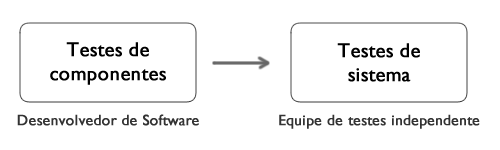
\includegraphics[width=8cm,scale=1]{images/f1.png}
\end{figure}
\par Os objetivos dos testes de componentes é achar, verificar se existem defeitos nos componentes do software, sejam eles funções, objetos, componentes reusáveis. Já o objetivo de testes de sistema está mais focado em descobrir defeitos da integração dos componentes, que são utilizados para formar subsistemas, também é verificado se o sistema atende aos requisitos funcionais e não funcionais para qual foi proposto \cite{SV07}.
\par Em \citeonline{SV07}, existem duas metas distintas sobre o processo de teste de software:
\begin{enumerate}
	\item Demonstrar ao desenvolvedor e ao cliente que o software produzido atende aos requisitos;
	\item Descobrir falhas ou defeitos no software produzido que apresenta comportamento incorreto, não desejável ou em não conformidade com sua especificação.
\end{enumerate}
\par Na primeira meta temos a validação do software, na qual esperamos que o software seja executado corretamente e faça o que se propõe. Na segunda meta expormos os defeitos, os testes são feitos exatamente para o software quebrar e não funcionar. Para o teste de validação, o resultado satisfatório é quando o software funciona corretamente, já para os testes de defeito, o resultado é considerado satisfatório quando o software mostra um defeito causando um funcionamento incorreto no sistema \cite{SV07}.
\par \citeonline{SV07} apresenta um modelo geral de processo de teste de software, vide figura abaixo:
\begin{figure}[htbp]
	\centering
	\caption{Modelo Geral de Processo de Teste de Software\label{fig:f2}. Fonte: \citeonline{SV07}}
	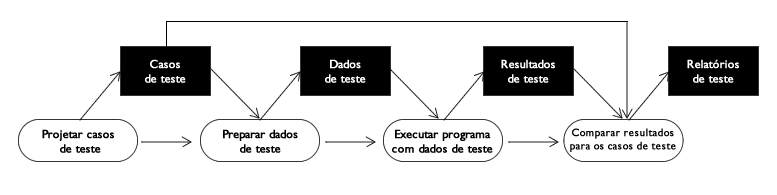
\includegraphics[width=16cm,scale=1]{images/f2.png}
\end{figure}
\par Os casos de teste são diretivas de entradas para o teste e as saídas esperadas, adicionado da descrição do que está sendo testado. Dados de teste são as entradas selecionadas para servir de entrada para os testes, em sua maioria gerados automaticamente através de softwares específicos. Nos resultados dos testes temos se as saídas esperadas foram alcançadas ou não, caso não tenham sido alcançadas, deve-se anotar qual o erro encontrado. No relatório de teste temos a junção de todos os casos de testes, suas entradas, saídas esperadas e saída alcançadas.
\par Geralmente são utilizados dois tipos de testes: teste de unidade e teste de aceitação.
\subsection{Testes de Unidade}
\par Testes de unidade são os escritos pelos desenvolvedores enquanto estes codificam o sistema, ou seja, aquela ideia inicial de deixar os testes para o final do projeto não vale aqui \cite{TL04}.
\par Os teste de unidade devem ser automatizados e todos devem rodar corretamente durante todo o processo de desenvolvimento do software, caso algum teste chegue a falhar, a prioridade da equipe de desenvolvimento passa a ser corrigir o código que está causando o erro. O grande objetivo dos testes de unidade, como Kent Beck falou, é garantir que o código gerado seja o mais limpo possível \cite{TL04}.
\par Uma das maiores vantagens no caso dos testes de unidade é que o desenvolvedor pensa no teste antes da implementação. Ele começa a entender os detalhes e as hipóteses de uso do código a ser produzido. Fazendo isso, o desenvolvedor está fazendo uma análise mais detalhada do problema. Ele deve codificar somente até o teste passar, nem mais, nem menos \cite{TL04}.
\subsection{Testes de Aceitação}
\par Os testes de unidade nos dão a segurança que as classes do nosso software estão funcionando perfeitamente, porém por mais que isso seja fundamental não é suficiente. Um requisito, estória ou funcionalidade pode utilizar mais de uma classe, e frequentemente são utilizadas mais de uma classe. Para isso existe os testes de aceitação, eles procuram simular a interação entre as classes, procuram simular também a interação do usuário com o software. Podemos dizer que o teste de aceitação é um roteiro de como agir e os resultados a esperar das ações desse roteiro \cite{TL04}.
\par Geralmente criada pelo cliente, ou pela equipe de negócio, pois estes conhecem bem a funcionalidade testada, são eles que conhecem e irão estabelecer quais os passos a serem efetuados naquela funcionalidade em questão. A execução dos testes de aceitação deve ser, preferencialmente, de forma automatizada. Sempre que for adicionada uma nova funcionalidade no software, os testes de aceitação devem ser escritos e testados, com isso no final, teremos uma suíte de testes de aceitação juntamente com os testes de unidade \cite{TL04}.
\par Diferente dos testes de unidade, os testes de aceitação não costumam ser executados com 100\% de acerto. Certamente a equipe terá que conviver com um percentual dos teste que não foram executados com sucesso. Geralmente defeitos nos testes de aceitação demoram um pouco mais e exigem mais esforços para serem reparados do que os testes de unidade.

\section{TDD - Desenvolvimento de Software Guiado a Teste}
\par O termo TDD foi apresentado por Kent Beck por volta de 1999, juntamente com termo Extreme Programming (XP) que advém das novas metodologias de desenvolvimento de software, conhecidas como Metodologias Ágeis.
\par O Extreme Programming é um processo de desenvolvimento de software que volta o foco do desenvolvimento para o cliente, através de diversas práticas dentre elas o TDD (Test Driven Development). O foco do XP é entregar um produto com maior valor em um curto espaço de tempo \cite{TL04}.
\par O termo TDD pode ser traduzido como Desenvolvimento de Software Guiado a Testes, o desenvolvedor antes de codificar seu código, ele escreve testes para guia-lo em seu desenvolvimento \cite{TL04}.
\par Segundo Teles (2004): 
\begin{citacao}
	Adotar o desenvolvimento guiado a testes é seguir o caminho da prevenção. O desenvolvedor incorpora alguns hábitos que irão assegurar que o seu software tenha uma probabilidade menor de contrair uma doença.
\end{citacao}
\par O TDD se apresenta em uma forma de ciclo, vide figura abaixo:
\begin{figure}[htbp]
	\centering
	\caption{Ciclo do TDD\label{fig:f3}. Fonte: Adaptada de \citeonline{KB2003}}
	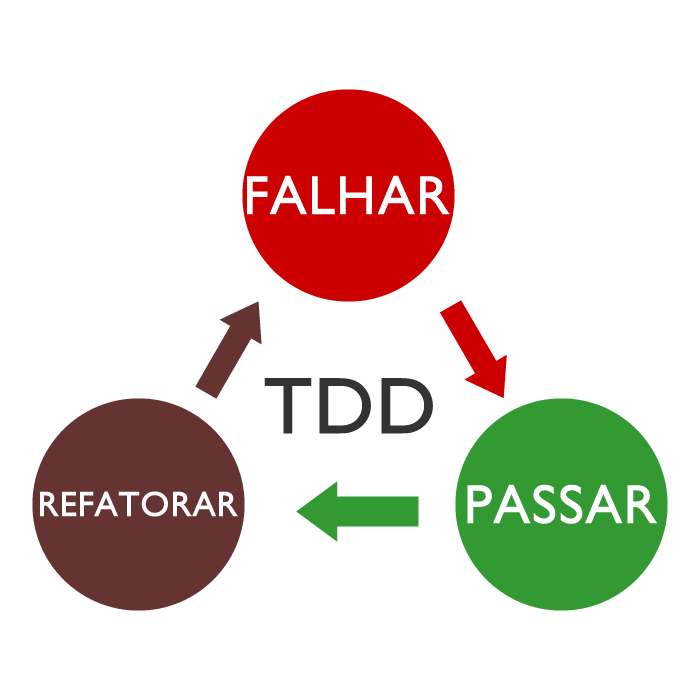
\includegraphics[width=8cm,scale=1]{images/f3.png}
\end{figure}
\begin{itemize}
	\item Na primeira fase, falhar (red), escrevemos um teste, devemos pensar como gostaríamos que a operação aparecesse em forma de código. Em seguida o desenvolvedor executa o teste, certamente ele irá falhar, pois ainda não foi desenvolvido nenhum código, somente o teste;
	\item Na segunda fase, passar (green), o objetivo do desenvolvedor agora é escrever um código que faça aquele teste ter o resultado esperado, ou seja passar, nem que seja de uma maneira rápida, é necessário fazer o teste passar;
	\item Na terceira fase, refatorar (refactor), o desenvolvedor volta para o seu código e o aprimora, utilizando os tipos de dados corretos, alterando as variáveis, enfim, fazendo mudanças que visem melhorar seu código no sentido computacional, em seguida o desenvolvedor refaz o teste.
\end{itemize}
\par O objetivo com isso é que no final o desenvolvedor tenha um código limpo e confiável \cite{KB2003}.

\chapter{Trabalhos Relacionados}
\par Nos últimos anos a comunidade acadêmica vem refletindo sobre a metodologia de ensino de fundamentos de programação, a fim de melhorar os índices e facilitar a aprendizagem do aluno. 
\par \citeonline{nor} em seu trabalho propõe uma nova metodologia para o desenvolvimento de sistemas de correção automática de listas de exercícios de programação, baseada em testes unitários. Trabalho este que visa a avaliação imediata do código escrito pelo aluno, sem o intermédio de um professor, isso força o aluno a se autoavaliar e corrigir os erros, caso os tenham. 
\par A metodologia aplicada por \citeonline{nor}, para implementação passa por 4 etapas:  na primeira etapa é selecionado um corpo de exercícios relacionados a um tópico dentro da disciplina, no momento posterior, o professor define quais as interfaces de cada função que deve ser implementada pelos alunos, sua entradas e saída, o próximo passo consistem em elaborar os testes de softwares para que o mesmo teste cada trecho do código que pedido no exercício, por fim, é solicitado ao aluno que implemente as funções da lista de exercícios e submeta o resultado à avaliação do sistema. 
\par \citeonline{nor} aplicou sua metodologia em uma turma de 70 alunos, onde foram desenvolvidas várias listas de exercícios e seus respectivos testes, uma para cada tema abordado. As listas foram entregues semanalmente, logo após cada tópico ser apresentado em sala de aula. Observou-se que o uso de testes agiu de forma incentivadora e motivador para o aprendizado dos alunos, que tiveram menos dificuldades em resolver os exercícios, já que o  tiveram um retorno imediato sobre a falha de seus códigos. Já fora da sala de aula, a correção automática, deu aos professores um ganho de tempo na correção dos mesmos, liberando-os para preparação de aulas novas e outras atividades acadêmicas. Um ponto negativo observado foi que as interfaces das classes e funções engessaram um pouco a codificação dos alunos. Outro ponto que observou-se foi que nem todos os testes foram implementados, dando a impressão que o aluno não soube ou não quis codifica-lo.
\par Em \citeonline{gom} é apresentado um ambiente que tem como objetivo principal auxiliar os alunos no processo de aprendizagem de fundamentos de programação. As principais funcionalidades elencadas para esse ambiente são: um módulo prático de ensino, um módulo teórico e um agente inteligente programado capaz de interagir com o aluno de acordo com o comportamento do mesmo.
\par \citeonline{gom} apenas apresenta o ambiente que vem sendo desenvolvido para auxiliar o ensino de programação, não foi colocado ainda esse ambiente em prática. Mas sua proposta busca não só o benefício para o aluno, bem como para os professores também, pois terão um feedback mais rápido dos alunos e poderão sugerir dicas e avaliar de formas mais rápida os alunos. \citeonline{gom} reflete que da forma como seu ambiente foi estruturado, a junção do teórico e prático, apoiados por um agente inteligente, pode estimular a resolução de problemas de uma forma lúdica e que atendam os requisitos esperado pela comunidade da área de ensino de fundamentos de programação.
\par Baseado em \citeonline{gom}, o trabalho aqui proposto também conta com um módulo prático e teórico, bem como uma interface para interação com o aluno, porém não está presente a funcionalidade de um agente inteligente. A interação deste trabalho se dá por uma interface web, na qual o aluno poderá consultar o material teórico, receber os teste, enviar o código para avaliação e receber de imediato a resposta do mesmo.
\par Outro trabalho que tem ganhado notoriedade no meio acadêmico e profissional é a iniciativa \citeonline{cod}. Trata-se de um plataforma web com uma proposta diferente de ensino de programação, onde o aluno interage com o sistema através de um console que processa instantaneamente os comandos enviados pelo aluno, muito semelhante ao console que ele encontra no próprio sistema operacional. São disponibilizados cursos como: Ruby, JavaScript, Python, Fundamentos de HMTL, JQuery e outros cursos. \par Atualmente o site está migrando para o idioma português, porém essa migração ainda não está completa. Para um acesso completo aos cursos é necessário fazer um registro simples, porém sem nenhum custo para o aluno. Os módulos das aulas são progressivos e bastantes intuitivos, o aluno vai avançando um passo de cada vez, como vimos nos baby-steps (passos de bebê). Também é possível criar um curso na plataforma \citeonline{cod}, porém até onde foi verificado, o curso criado será avaliado pelos administradores da plataforma antes de ser disponibilizados.
\par \citeonline{TF12} traz um trabalho bastante completo envolvendo Desenvolvimento Guiado a Testes e ensino de programação, em seu trabalho, disponilizado através de um site, temos dois cursos disponíveis, um para aprender a linguagem Ruby e um para Javascript, duas linguagens em ascensão no momento. Também no site \citeonline{TF12} disponilizou um vídeo onde mostra como funciona o uso de testes na linguagem Ruby. As aulas são distribuídas através de um único arquivo compactado que contém todo o conteúdo do curso. O método de \citeonline{TF12} é para o ensino auto-didata, sem um auxilio do professor. Em resumo, a pessoa que quiser aprender pelo método \citeonline{TF12}, deve ir ao site, assistir ao vídeo, fazer o download do arquivo com as aulas e depois ler e praticar sozinho. Vale salientar que todo o conteúdo de \citeonline{TF12} está em inglês.

\chapter{Procedimentos metodológicos}
\par A metodologia utilizada para esse trabalho consiste de etapas: 
\begin{itemize}
	\item selecionar conteúdo didático;
	\item configurar a ferramenta;
	\item ministrar um curso;
	\item aplicar um questionário pós-teste;
	\item avaliar os resultados do curso.
\end{itemize}
\section{Selecionar conteúdo didático}
\par Foi realizada uma entrevista (em Anexo I) com os professores que lecionam as disciplinas de fundamentos de programação no Campus da Universidade Federal do Ceará, campus Quixadá, afim de averiguar quais as dificuldades dos alunos e quais os conteúdos mais relevantes. Os conteúdos didáticos escolhidos foram: Operações Matemáticas, Literais (String, char), Variáveis, Subprogramas (Métodos e funções),  Controle de fluxo(If/else, switch), Laços de repetição(for, while), e Agrupamento de valores(Array). 

\par Na fase de escrever os testes, foram selecionados exercícios que abordassem o conteúdo apresentado na sala de aula. Para facilitar a implementação dos testes, foram utilizados o framework Rspec, devido a sua facilidade de manuseio e sua boa documentação.
\section{Configurar a ferramenta}
\par Depois de elaborar o conteúdo e os seus respectivos testes, os mesmo são disponibilizados para os alunos via ferramenta que foi elaborada neste trabalho. Neste trabalho aqui apresentado, o conteúdo foi pensado anteriormente e os testes foram escritos antes, bem como \citeonline{nor}, porém não houve uma seleção de um corpo de exercícios, já que a linguagem utilizada no curso se trata de outra diferente e não da que é aplicada na realidade do Campus Quixadá.
\section{Ministrar um curso}
\par O curso será aplicado aos alunos da Universidade Federal do Ceará, campus Quixadá, que tenham dificuldades com fundamentos de programação, sejam eles, repetentes de alguma disciplinas de fundamentos ou não. 

\par O curso terá uma duração de 8 horas, onde será destinado um tempo para abordar o conteúdo teórico e depois teremos a prática. A parte prática contará com um servidor que estará recebendo os arquivos dos alunos e processando o resultado dos teste em cima de cada exercício que os alunos enviarem. O professor poderá acompanhar em tempo real como os alunos estão se saindo em cada um dos exercícios.

\par Tanto a parte teórica, quanto a parte prática será acessível apenas pela ferramenta. A ideia de ambiente integrado é um conceito importante para a implementação deste trabalho, pois une um pouco de tudo que está relacionado com o ensino de sala de aula.
\section{Aplicar um quetionário pós-teste}
\par Foi elaborado um questionário pós-teste (em Anexo I) de cunho qualitativo com a finalidade de extrair a impressão dos alunos sobre a ferramenta e o método de ensino. Este questionário será aplicado aos alunos no final do curso.
\section{Avaliar os resultados do curso}
\par Na fase de análise de dados, será realizado um levantamentos dos dados obtidos através das respostas do questionário pós-teste. 

\chapter{A Ferramenta}
\section{Introdução sobre a ferramenta}
\par A ferramenta foi desenvolvida com o objetivo de auxiliar no processo de ensino e aprendizado de fundamentos de programação. A ferramenta possui um módulo prático onde o aluno pode ver quais são os exercícios passados através de testes de software e no qual ele pode submeter o seu código para avaliação, bem  como o módulo teórico, que traz o conteúdo teórico com exemplos e dicas relacionadas a cada conteúdo. 
\par O módulo prático traz a tona uma questão bastante requisitada, tanto por alunos, quanto por professores, que é o feedback. A cada exercício resolvido o aluno irá submeter seu código produzido e terá do sistema uma resposta que irá mostrar se o aluno acertou ou errou. Caso o aluno erre, ele pode refatorar seu código e mandar novamente, quantas vezes forem necessárias para que chegue ao sucesso.
\par O objetivo do módulo teórico é que o aluno tenha acesso a um material mais refinado possível, facilitando o acesso do aluno ao que realmente importa nos conceitos.  No módulo teórico deve ser ofertada uma visão completa do que o aluno deve aprender de conceitos, o conteúdo que estará disponível para o aluno é de responsabilidade do professor, ou seja, o professor terá que preencher cada aula com o seu respectivo conteúdo.
\par Afim de ilustrar como será o uso da ferramenta, segue abaixo um cenário de uso que mostra como o aluno e o professor interagem com a ferramenta.
\section{Cenário de Uso}
\par "João e Pedro, são respectivamente professor e aluno do curso de fundamentos de programação da Universidade de Computação Computacional. João anda bastante preocupado com o alto índice de desistência dos alunos do curso e com o alto índice de reprovação. Pensando em mudar um pouco o foco da disciplina ele resolveu utilizar a metodologia e a ferramenta aqui proposta nesse trabalho. João inicialmente solicita ao administrador do sistema que crie um curso para ele com o nome de “Fundamentos de Programação com Ruby”, o administrador cria o curso e deixa sobre a responsabilidade de João. João começa a criar aulas e colocar o conteúdo nelas, inclusive os arquivos de testes que serão necessários para os alunos checarem seus códigos. João avisa a Pedro que está utilizando agora uma ferramenta e pede para Pedro se cadastrar nessa ferramenta e avisar aos demais alunos para que faça o mesmo. Pedro, como é um aluno exemplar, se cadastra sem problemas no sistema e avisa a João que fez o que ele pediu." 
\par "João agora pode adicionar Pedro e os demais alunos ao seu curso. Então, depois de adicionados os alunos ao curso, os mesmos poderão consultar todo conteúdo das aulas. Pedro ler o conteúdo teórico da primeira aula e se sente motivado a tentar passar pelo primeiro teste. Pedro, vê o teste e resolve escrever um programa que faça passar por aquele teste, ele então submete a avaliação, porém, para surpresa de Pedro, seu código não passou. Foi mostrada a Pedro uma mensagem de erro na segunda linha de seu código, Pedro não desanima e corrige o erro e envia novamente o seu código para uma nova avaliação, dessa vez Pedro teve sucesso e passou por esse teste. Pedro continua para o próximo conteúdo, ler e aprende o conceito e segue com o ciclo de tentativa e erro até terminar todos os testes do conteúdo do curso."
\section{Funcionalidades}
\par As funcionalidade da ferramenta foram baseadas em papéis do cotidiano real de uma sala de aula, com exceção do Administrador, são eles o Aluno e o Professor.
\subsection{Administrador}
\par Esse papel é responsável por todo o controle de todas existentes no sistema, somente ele pode cadastrar novos cursos.
\begin{figure}[htbp]
	\centering
	\caption{Tela inicial do Administrador\label{fig:tela-adm}. Fonte: Próprio autor}
	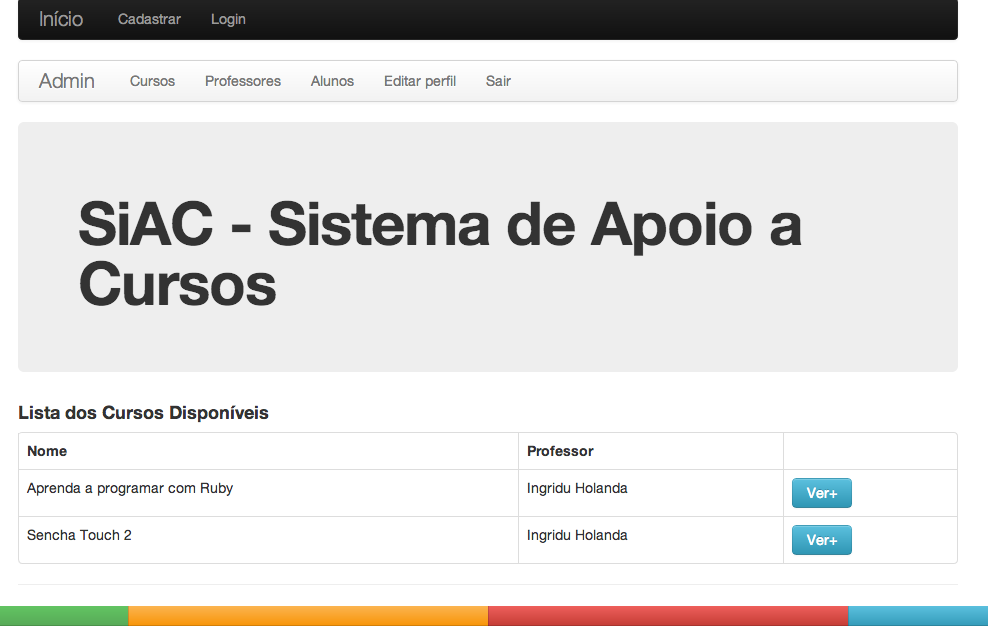
\includegraphics[width=8cm,scale=1]{images/tela-adm.png}
\end{figure}
\begin{figure}[htbp]
	\centering
	\caption{Diagrama de Caso de Uso do Adminstrador\label{fig:dia-adm}. Fonte: Próprio autor}
	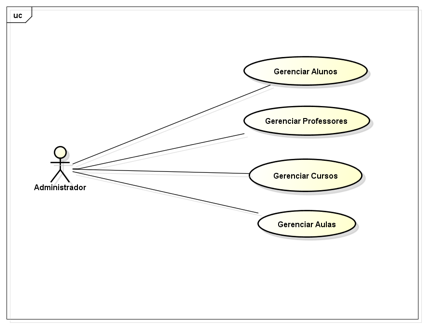
\includegraphics[width=8cm,scale=1]{images/dia-adm.png}
\end{figure}
 
\subsection{Professor}
\par Assim como no ambiente de sala de aula, o professor é responsável em adicionar e alterar as aulas. Cada aula que o professor colocar ele poderá adicionar um arquivo de teste, que será utilizado pelos alunos para servir de guia para os seus códigos. O professor também poderá adicionar e remover alunos aos seus cursos. Ele pode também alterar seus dados pessoais.
\begin{figure}[htbp]
	\centering
	\caption{Tela inicial do Professor\label{fig:tela-prof}. Fonte: Próprio autor}
	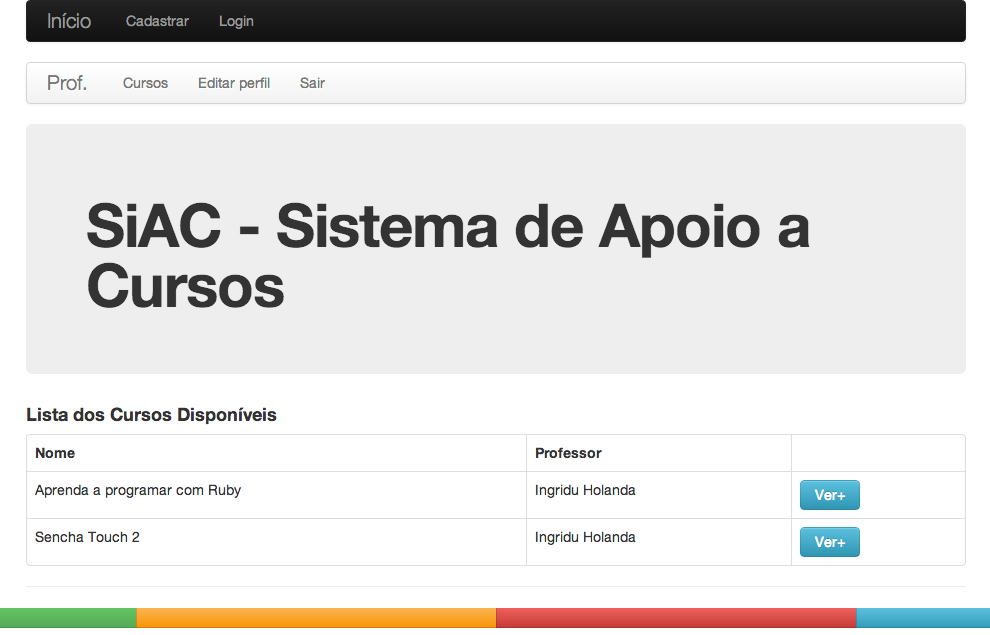
\includegraphics[width=8cm,scale=1]{images/tela-prof.png}
\end{figure}
\begin{figure}[htbp]
	\centering
	\caption{Diagrama de Caso de Uso do Professor\label{fig:dia-prof}. Fonte: Próprio autor}
	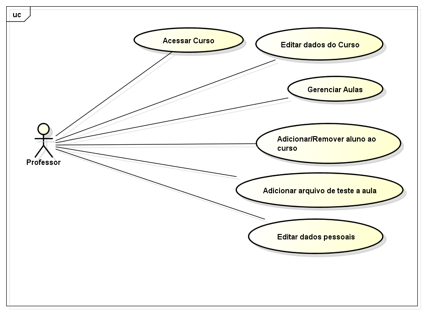
\includegraphics[width=8cm,scale=1]{images/dia-prof.png}
\end{figure}
 
\subsection{Aluno}
\par O aluno poderá participar de um ou mais cursos e ter acesso as suas respectivas aulas, cada aula poderá conter um arquivo de teste, caso o tenha, o aluno poderá fazer download do arquivo. O aluno também poderá enviar seu código para avaliação do sistema, no caso, o mesmo será corrigido instantaneamente e será retornada uma mensagem de erro ou acerto. O aluno poderá enviar o código quantas vezes forem necessárias até atingir o acerto. Ele pode também alterar seus dados pessoais.
\begin{figure}[htbp]
	\centering
	\caption{Tela inicial do Aluno\label{fig:tela-alu}. Fonte: Próprio autor}
	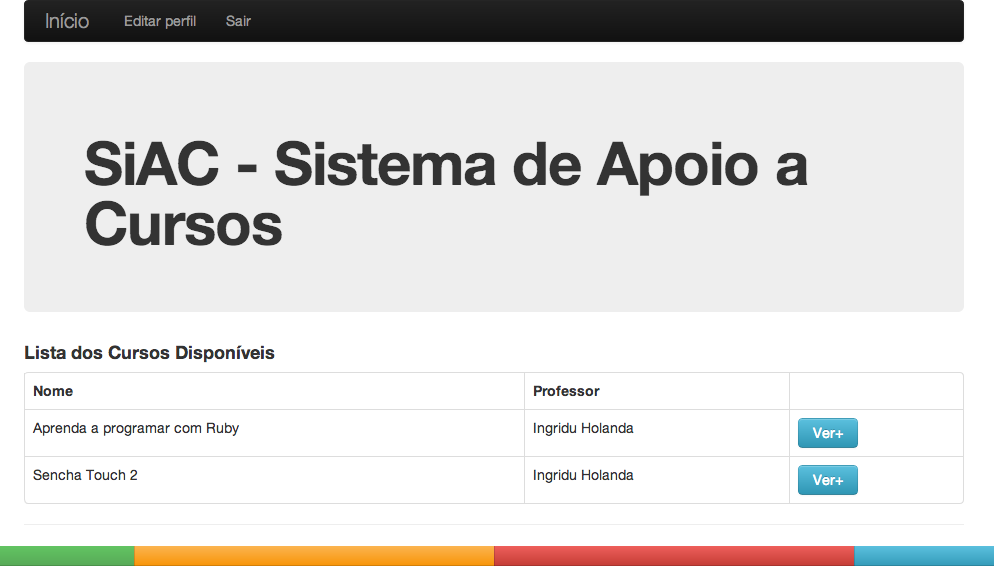
\includegraphics[width=8cm,scale=1]{images/tela-alu.png}
\end{figure}
\begin{figure}[htbp]
	\centering
	\caption{Diagrama de Caso de Uso do Aluno\label{fig:dia-alu}. Fonte: Próprio autor}
	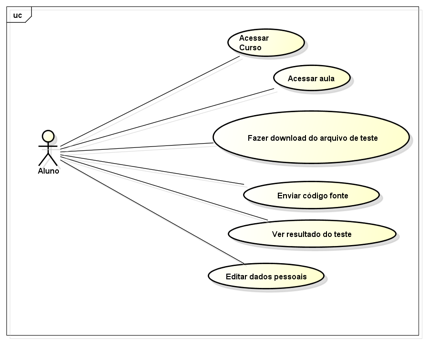
\includegraphics[width=8cm,scale=1]{images/dia-alu.png}
\end{figure}
 
\section{Arquitetura e Implementação}
\par A arquitetura proposta para a implementação do sistema está estruturada sobre o padrão de projeto MVC (Model, View, Controller), onde há uma camada responsável pela apresentação/visualização do sistema, uma camada de negócio, onde será implementada as regras de negócio da aplicação e uma camada de modelos, onde temos as entidades envolvidas e a comunicação com o banco de dados. 

\par A camada de visão faz fronteira do usuário com a ferramenta, a partir da mesma são geradas as ações pretendidas pelo usuário. Essas ações são capturas e processadas pela camada de controle, que requisita a camada de modelo para trazer/enviar informações das entidades envolvidas na ação e a mesma se comunica com o banco para recuperar/armazenar os dados.
\begin{figure}[htbp]
	\centering
	\caption{Padrão MVC em Ruby on Rails\label{fig:mvc}. Fonte: Próprio Autor}
	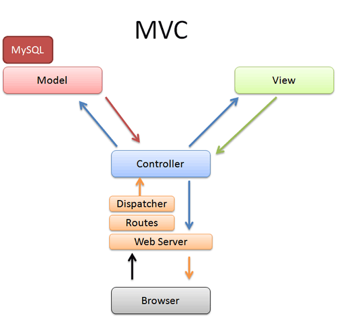
\includegraphics[width=8cm,scale=1]{images/mvc.png}
\end{figure}
\par A implementação da ferramenta foi sobre a linguagem Ruby, versão 1.9, juntamente com o framework Rails(http://rubyonrails.com.br/), versão 3.2, para prover desenvolvimento do portal web. O ambiente escolhido para interação do usuário é o ambiente web, por não necessitar de uma instalação por parte do usuário, basta ter um programa navegador de internet para utilizar a ferramenta.
\par Para fazer com que o código do enviado pelo aluno fosse testado, foi utilizado o framework Rspec(http://rspec.info/). A implementação se deu da seguinte maneira: o aluno envia o arquivo com extensão .rb, o servidor recebe o arquivo, confirma se realmente se trata de um arquivo Ruby, caso não, um alerta será mostrado ao usuário, caso contrário o servidor irá renomar o arquivo para "codigo.rb". Em seguida a ferramenta copia o código enviado pelo aluno e o arquivo de teste para uma pasta temporária, onde será realizada o teste, feito o teste, é gerado um arquivo de log, onde fica o resultado do teste. A ferramenta por sua vez, lê o arquivo de log, copia os dados e salva no banco de dados, passando a referência do aluno, da aula e do teste.
\par Os frameworks utilizados, além do Rails, foram o Paperclip(https://github.com/thoughtbot/paperclip), que gerencia o envio de arquivos, o Ckeditor(http://ckeditor.com/), que provê uma interface mais amigável na hora de editar o conteúdo, o Bootstrap(http://twitter.github.com/bootstrap), que facilita a montagem das páginas e dá uma visualização melhor, trazendo boas práticas de IHC e o Devise(https://github.com/plataformatec/devise), que abstrai a camada de autenticação e autorização, tornando mais fácil a implementação dos vários papéis de usuários que temos na aplicação. Os frameworks relacionados a testes que foram utilizados foram o Minitest(https://github.com/seattlerb/minitest) e o Rspec, que juntos fazem a validação e verificação do código gerado pelo aluno.
\par O banco de dados utilizado inicialmente será o SQLite, pois se trata de um banco simples e de fácil manutenção. Em um momento posterior, cogita-se mudar o banco para um que ofereça suporte completo ao SQL, visto que a grande massa de dados que serão alocadas precisa ser tratada com mais agilidade e optimização.
\par Alguns casos de usos foram pensados, porém não implementados, como por exemplo um terminal interativo, onde o aluno poderia codificar na própria ferramenta, sem a necessidade de enviar o arquivo, o que facilitaria mais ainda a interação do aluno. Por questões de tempo e prioridade, tal funcionalidade foi deixada para um momento posterior.

\chapter{Resultados do Experimento}
\par Com o intuito de verificar a opinião e como foi a experiência dos alunos com a metodologia e a ferramenta, foi aplicado um questionário após a realização do curso.

\par Este questionário foi aplicado a 6 alunos dos cursos de Sistemas de Informação e Engenharia de Software da Universidade Federal do Ceará que estavam presentes no curso. Os alunos do curso já tinham alguma vivencia com programação, porém nunca tiveram contato com a linguagem quem foi utilizada no curso.

\par Primeiramente foi observado que os alunos entenderam a principal ideia da metodologia, que foi a figura dos testes como forma de aprendizagem, errado, corrigindo e por fim acertando, outro ponto que ficou bem evidente foi que os mesmos se mostraram atentos em consultar o material que ficou disponível na ferramenta. Os passos da metodologia e o uso da ferramenta foram bem transmitidos e bem entendido pelos alunos.

\par Voltando o olhar agora para a ferramenta, com relação ao conteúdo e a forma como ele foi apresentado aos alunos, pude constatar que a maioria dos alunos achou o conteúdo simples e sem muita dificuldade de consultar, ficou visível que eles utilizaram o conteúdo para uma consulta mais a fundo. O conteúdo continha os tópicos principais de cada assunto juntamente com alguns exemplos de códigos, a maioria dos alunos conseguiu visualizar ambos sem problemas.

\par A ferramenta do ponto de vista de usabilidade mostrou-se muito fácil de utilizar, com botões grande e informativos, o uso de cores vivas, fontes de tamanhos destacados, distribuição dos elementos na página, favoreceram a experiência e a usabilidade da ferramenta pelos alunos. Algumas mensagens de erros não foram tratadas visualmente, o que confundiu um pouco alguns alunos, porém nada que influenciasse no uso pleno da ferramenta.

\par Como dito anteriormente, a linguagem escolhida para ser ministrada no curso foi Ruby, por se tratar de uma linguagem que não exige tanto da sintaxe. Como nenhum dos alunos tiveram a oportunidade de programar em Ruby anteriormente, muitos ficaram surpresos com a facilidade sintática da linguagem, todos os alunos gostaram da linguagem e demonstraram que aprenderam rapidamente sem nenhuma barreira.

\par Os pontos positivos tanto da ferramenta quanto do curso foram a maneira como o curso foi conduzido, por mais rápido que tenha sido, e a facilidade em utilizar a ferramenta. Foi bastante proveitoso o uso da ferramenta pois não foi necessário instalar ou configurar qualquer tipo de ambiente de programação na máquina dos alunos, o que facilitou e agilizou o curso.

\par Já com relação aos ponto negativos, infelizmente o curso foi ministrado em pouco tempo e os alunos ficaram ansiosos por mais aulas e mais conteúdo. Outro ponto que precisa melhorar foi a forma com que a ferramenta apresenta o resultado aos alunos, por nunca terem visto a forma de programar orientado a testes e não conhecerem os testes de software, muitos alunos não entenderam, em um primeiro momento, os resultados ali apresentados. O que poderia ser feito seria uma pré-aula mostrando como o desenvolvimento guiado a teste funciona e como analisar o código. A funcionalidade de anexar arquivos ao conteúdo da aula também fez falta, haja visto que os alunos solicitaram os slides da apresentação.

\par No geral essa análise trouxe alguns aspectos que precisamos fortalecer e outros pontos que precisamos melhorar, também foram analisadas algumas funcionalidades que não foram implementadas na ferramenta mas que seriam interessantes de serem implementadas na próxima versão.


\chapter{Considerações Finais}

\par Neste trabalho aqui apresentado foi proposta uma ferramenta que juntamente com a metodologia visam melhorar a experiência do ensino de fundamentos de programação. Esse método e a ferramenta podem auxiliar tanto o aluno quanto o professor, pois facilitar o feedback de ambos com relação a como o aluno está progredindo na disciplina. A aproximação dos alunos com o teste de software também é uma das consequências desse trabalho, visto que o aluno vai está aprendendo voltado a desenvolver código que passe nos testes que o professor disponibilizou.

\par As principais dificuldades enfrentadas para que esse trabalho acontecesse primeiro foi a implementação da ferramenta, pois a mesma deveria testar um código enviado pelo aluno e retornar a ele uma resposta. Foram utilizadas diversos frameworks de teste de software utilizando Ruby, até se chegar ao desejado, depois disso o desafio foi fazer com que o servidor rodasse o código do aluno juntamente com o arquivo de teste do professor.
\par Preparar as interfaces visuais também foi um desafio que não pode ser esquecido. Todas as telas e os princípios de IHC foram aplicados nas interfaces para que o aluno tivesse a melhor experiência possível na ferramenta. Não o deixando confuso na hora de escolher as opções disponíveis. O foco aqui era não fazer com que o aluno perdesse a concentração no conteúdo e no curso e ficasse em conflito com a interface.

\par Outros problemas surgiram na fase de seleção e aplicação do curso, isto porque, tiveram que ser remarcado várias vezes por questões de não ter um público ideal disponível, infelizmente a aplicação do curso não saiu como o esperado, esperava-se uma turma de mais ou menos 15 a 20 alunos e tivemos apenas 6 estudantes que participaram do curso, mas nem por isso, o curso deixou de ser proveitoso para o que participaram,. 


\section{Trabalhos Futuros}
Para trabalhos futuros, foi pensado um refinamento da ferramenta baseado nos resultados do experimento, adição de um console interativo na ferramenta, para que o aluno não precisa utilizar outro programa qualquer, apenas o navegador de internet. Uma nova forma de aplicar o curso, separando os alunos em dois grupos, um que utilizará a ferramenta e o método e outro que não utilizara nada, apenas as aulas normais. No grupo que utilizasse a ferramenta e o método teríamos a adição de mais um questionário pré-teste (em Anexo I) com o objetivo averiguar qual o nível de conhecimento do aluno em fundamentos de programação. Esse mesmo questionário seria aplicado para mesma turma ao final do curso, afim de checar se houve ou não um aprendizado sobre o que foi exposto no curso. Ao final do curso, fazer um comparativo entre os dois grupos, conferindo se a ferramenta e o método se mostraram eficazes no aprendizado de fundamentos de programação.



\bibliographystyle{abnt-alf}
\bibliography{bib}
\end{document}
